\section{A section}

\begin{frame}{\insertsectionhead}
  
  ``Movement of a motile cell or organism, 
  or part of one, 
  in a direction corresponding to 
  a gradient of increasing or decreasing concentration 
  of a particular substance.''
  
  \vspace*{9pt}
  
  \begin{itemize}
    \item Directed movement of cells tends to be in response to 
    signalling molecules, 
    released by other cells in minuscule amounts
    \begin{itemize}
      \item E.g. 
      Development of tissue and organs, 
      Immune system cell response to pathogens
    \end{itemize}
  \end{itemize}
  
  \vspace*{9pt}
  
	\underline{Do cells respond in a similar way to electrical fields?}
  
\end{frame}


\subsection{Subsection}

\begin{frame}{\insertsubsectionhead}
  
  E.g. E. Coli 'run and tumble' motion

	\begin{figure}[h!]
    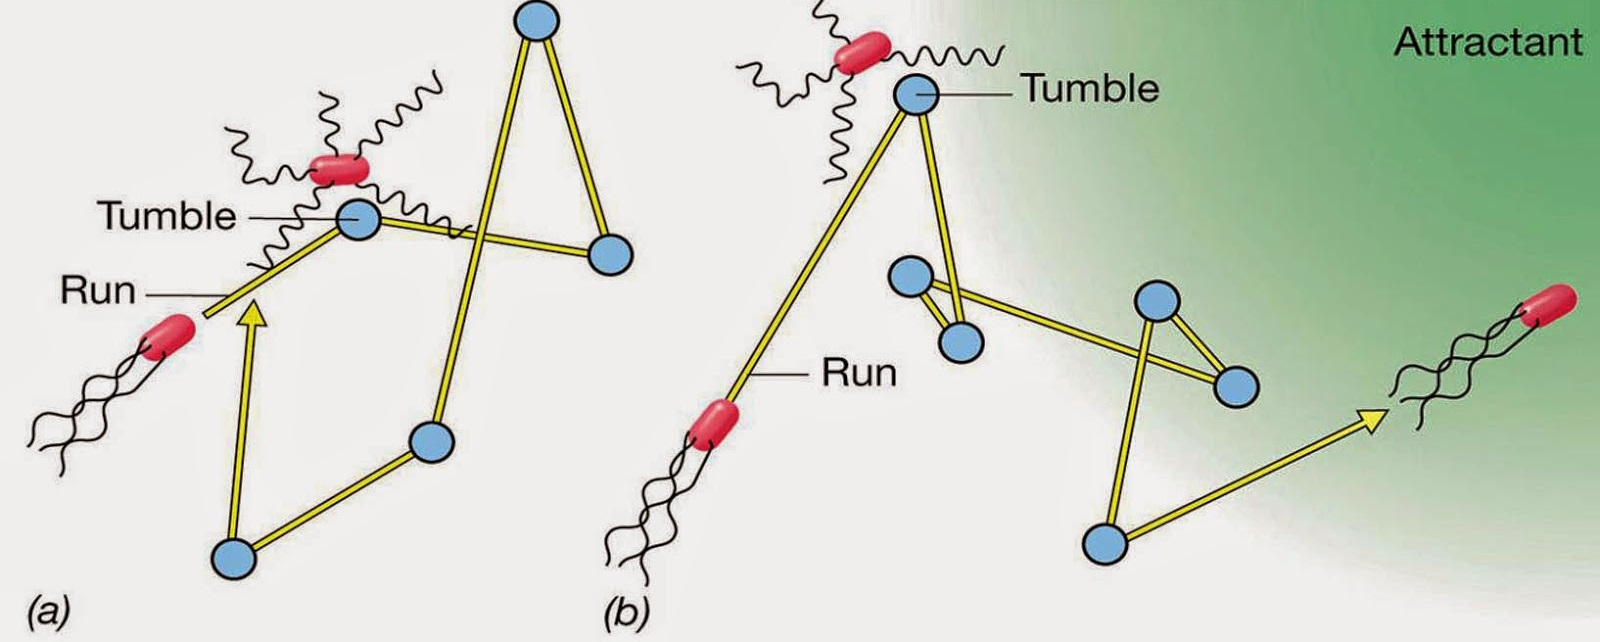
\includegraphics[width=0.7\textwidth]{src/img/example0}
		\caption{E. Coli chemotaxis}
		\source{\url{http://biologicalexceptions.blogspot.co.uk/2014/09/}}
  \end{figure}
  
	\begin{itemize}
    \item Cell swims in a direction and 
      randomly change direction after 
			'tumbling' at random times
		\begin{itemize}
      \item Direction chosen is biased towards 
        positive nutrient gradients
		\end{itemize}
	\end{itemize}

\end{frame}


\begin{outline}

  THINGS TO TALK ABOUT :
  \begin{itemize}
    \item CELLS AND STUFF
    \item E.COLI AND RUN-AND-TUMBLE
  \end{itemize}

\end{outline}


\subsection{Another subsection}

\begin{frame}{\insertsubsectionhead}

  But not all motile cells have flagella..
  
  \begin{figure}
    
		\begin{subfigure}{0.4\textwidth}
			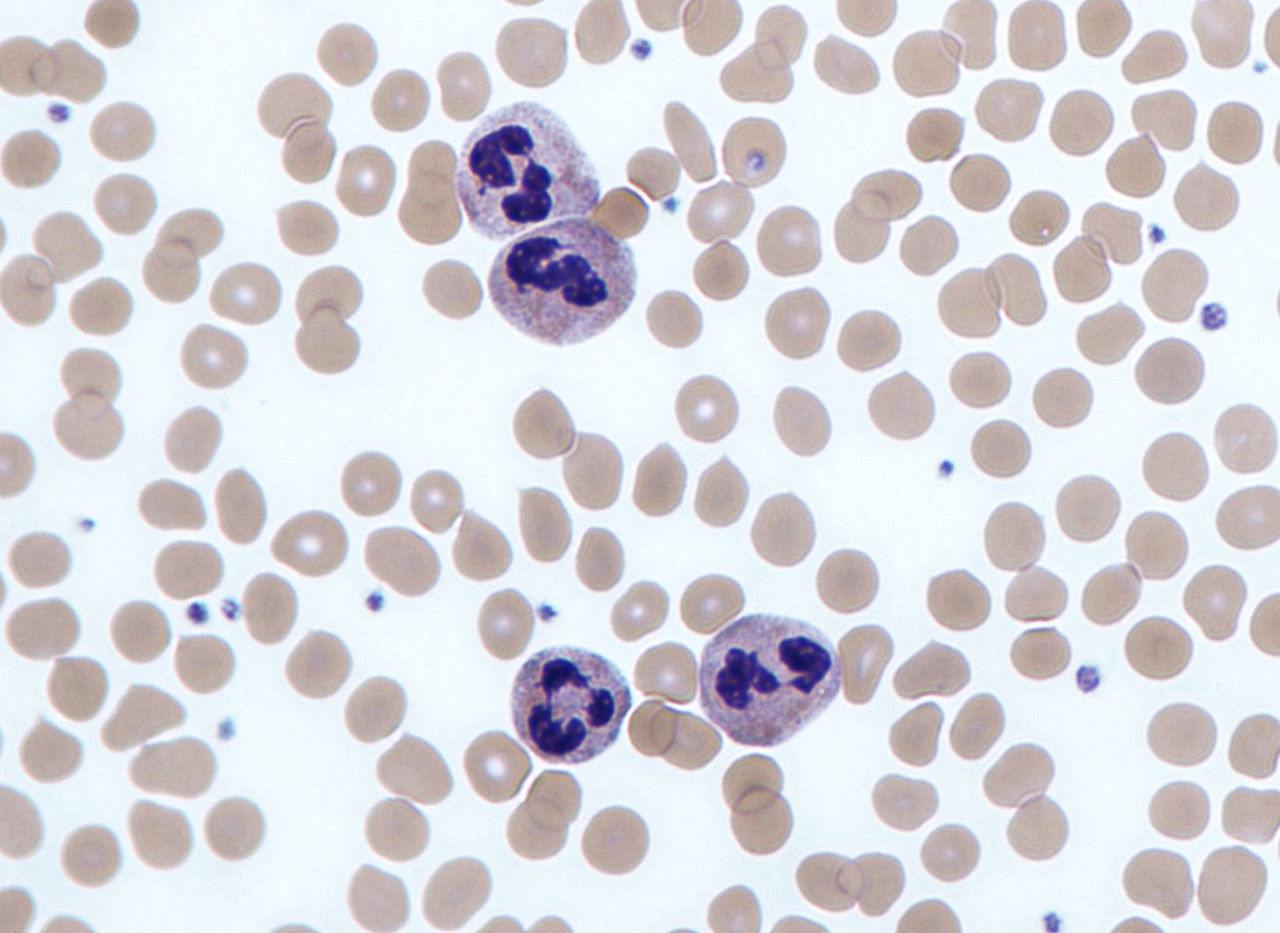
\includegraphics[width=\textwidth]{src/img/example1}
			\caption{White blood cells}
		\end{subfigure}
		\begin{subfigure}{0.44\textwidth}
			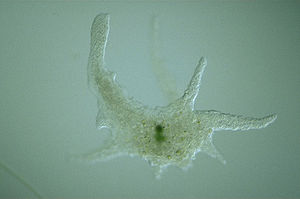
\includegraphics[width=\textwidth]{src/img/example2}
			\caption{Amoeba}
		\end{subfigure}
    
    \source{
      Wikipedia entries, 
        \textit{Neutrophil}, 
        and \textit{Chaos (genus)},  \\
      \url{https://en.wikipedia.org/wiki/File:Neutrophils.jpg}  \\
      \url{https://en.wikipedia.org/wiki/File:Chaos_carolinense.jpg}
    }
	\end{figure}

\end{frame}

\begin{frame}{Differently named frame}

  But not all motile cells have flagella..
  
  \begin{figure}
    
		\begin{subfigure}{0.4\textwidth}
			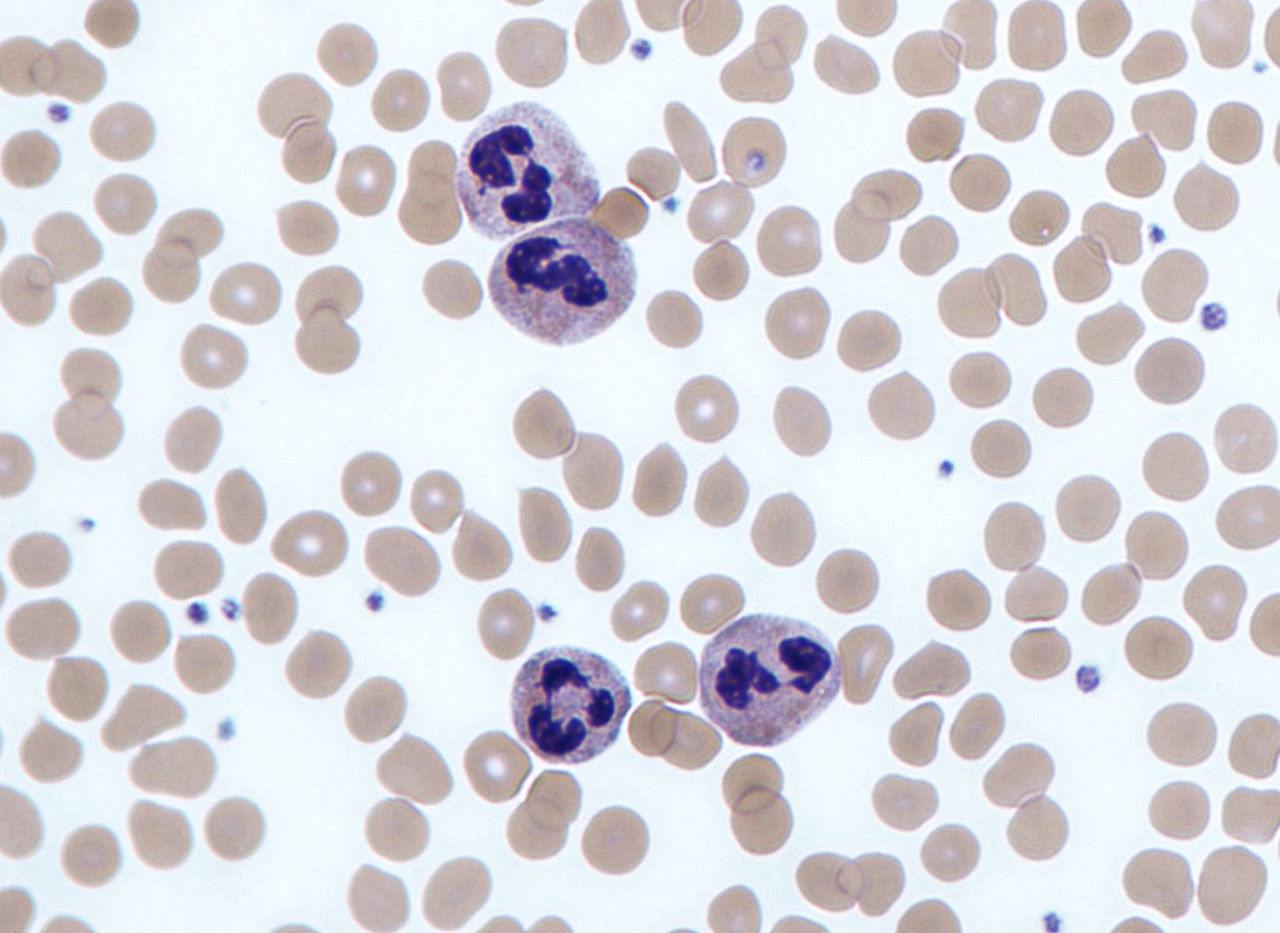
\includegraphics[width=\textwidth]{src/img/example1}
			\caption{White blood cells}
		\end{subfigure}
		\begin{subfigure}{0.44\textwidth}
			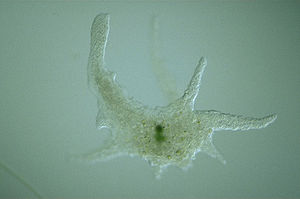
\includegraphics[width=\textwidth]{src/img/example2}
			\caption{Amoeba}
		\end{subfigure}
    
    \source{
      Wikipedia entries, 
        \textit{Neutrophil}, 
        and \textit{Chaos (genus)}, 
      \url{https://en.wikipedia.org/wiki/File:Neutrophils.jpg}  
      \url{https://en.wikipedia.org/wiki/File:Chaos_carolinense.jpg}
    }
	\end{figure}

\end{frame}